%This is a template download. 
% Original author:
% Spencer Shaw

\documentclass[paper=a4, fontsize=11pt]{scrartcl} % A4 paper and 11pt font size

\usepackage[T1]{fontenc} % Use 8-bit encoding that has 256 glyphs
\usepackage{fourier} % Use the Adobe Utopia font for the document - comment this line to return to the LaTeX default
\usepackage[english]{babel} % English language/hyphenation
\usepackage{amsmath,amsfonts,amsthm} % Math packages

\usepackage{lipsum} % Used for inserting dummy 'Lorem ipsum' text into the template

\usepackage{sectsty} % Allows customizing section commands
\allsectionsfont{\centering \normalfont\scshape} % Make all sections centered, the default font and small caps
\usepackage{graphicx}
\usepackage{fancyhdr} % Custom headers and footers
\pagestyle{fancyplain} % Makes all pages in the document conform to the custom headers and footers
\fancyhead{} % No page header - if you want one, create it in the same way as the footers below
\fancyfoot[L]{} % Empty left footer
\fancyfoot[C]{} % Empty center footer
\fancyfoot[R]{\thepage} % Page numbering for right footer
\renewcommand{\headrulewidth}{0pt} % Remove header underlines
\renewcommand{\footrulewidth}{0pt} % Remove footer underlines
\setlength{\headheight}{13.6pt} % Customize the height of the header

\numberwithin{equation}{section} % Number equations within sections (i.e. 1.1, 1.2, 2.1, 2.2 instead of 1, 2, 3, 4)
\numberwithin{figure}{section} % Number figures within sections (i.e. 1.1, 1.2, 2.1, 2.2 instead of 1, 2, 3, 4)
\numberwithin{table}{section} % Number tables within sections (i.e. 1.1, 1.2, 2.1, 2.2 instead of 1, 2, 3, 4)

\setlength\parindent{0pt} % Removes all indentation from paragraphs - comment this line for an assignment with lots of text

%----------------------------------------------------------------------------------------
%	TITLE SECTION
%----------------------------------------------------------------------------------------

\newcommand{\horrule}[1]{\rule{\linewidth}{#1}} % Create horizontal rule command with 1 argument of height

\title{	
\normalfont \normalsize 
\textsc{Georgia Institute of Technology - Guggenheim School of Aerospace Engineering} \\ [25pt] % Your university, school and/or department name(s)
\horrule{0.5pt} \\[0.4cm] % Thin top horizontal rule
\huge System Dynamics Notes \\ % The assignment title
\horrule{2pt} \\[0.5cm] % Thick bottom horizontal rule
}

\author{Spencer Shaw} % Your name

\date{\normalsize\today} % Today's date or a custom date

\begin{document}

\maketitle % Print the title

%----------------------------------------------------------------------------------------
%	PROBLEM 1
%----------------------------------------------------------------------------------------

\section{Modeling Mechanical Systems}

Systems can be described in units of Length, Mass or Time. Measurement systems can be 'absolute' or 'gravitational'. In absolute systems, Mass is chosen as a primary dimension, and force is a derived quantity. In this system, force is defined from mass and acceleration F = ma. In gravitational systems, Force is a primary dimension. In gravitational systems, mass is defined from the ratio of the Force on an object to its acceleration. Mass is defined as $\frac{F}{a}$. SI units are an example of an absolute measurement system (kg, m, s). The British Engineering System (BES) is an example of a gravitational measurement system (lbf, ft, s). All examples will be given in SI units. A chart comparing aboslute and gravitational systems can be found in the appendix.\\

Mechanical Systems are made up of 3 primary elements. 
\begin{itemize}
\setlength\itemsep{0em}
\item Springs: Elements that exert a force/torque proportional to their displacement
\item Dampers: Elements that oppose the direction of motion 
\item Inertial elements: Masses and their moments of inertia. \\
\end{itemize} 

In our diagrams we use the following notation conventions: 
\begin{itemize}
\setlength\itemsep{0em}
\item Capital Letters (X, Y, Z): Positions of elements naturally extended.
\item Letter P: Location of an acting force.
\item Lower Case Letters (x, y, z): Displacement from an origin or natural length.\\
\end{itemize}



\subsection{Elemental Behavior}

\subparagraph{Springs}~ \\
A Linear spring is one whose displacement is proportional to an applied outside force. If a force is acting on a linear spring, the following is true: 
$$F \propto x$$

Using empirical values we can determine the spring constant, k, as follows:
$$k = \frac{F}{x}$$
$$F = kx$$
Consider a spring lengthened by an outside force. Due to Newtons 3rd law, the spring will apply and equal and opposite force on its surroundings. If a spring is lengthened, the spring will apply a force on its surroundings towards its center. If the spring is compressed, it will apply a force on its surroundings away from its center. A force is 'positive' if it points towards the center of the spring. A force is 'negative' if it points away from the center of the sping.\\

\begin{figure}
\begin{center}
  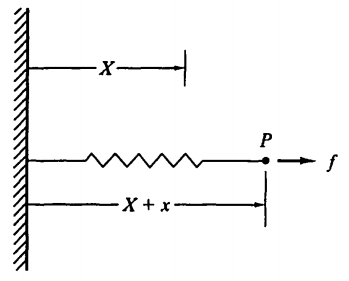
\includegraphics[width=17em]{Linear_Spring_1.png}
  \caption{Example of a Linear Spring}
  \label{fig:boat1}
\end{center}
\end{figure}

A Linear Torsional Spring is one whose displacement is proportional to a torque applied on it by the environment. This is a rotational displacement. \\
$$\tau \propto \theta$$
Using empirical values, we can determine a spring constant, k, as follows:
$$k = \frac{\tau}{\theta}$$
$$\tau = \frac{k}{\theta}$$

\begin{figure}
\begin{center}
  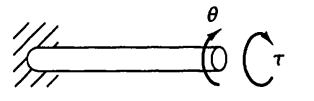
\includegraphics[width=17em]{Torsional_Spring_1.png}
  \caption{Example of a Torsional Spring}
  \label{fig:boat1}
\end{center}
\end{figure}
Springs store potential energy. The potential energy of a spring can be found using the following: \\
$$PE = \frac{1}{2} kx^2$$

\subparagraph{Dampers}~ \\
A Damper is a mechanical element that opposes motion. While springs can be used to store potential energy, a damper is used to dissipate kinetic energy as heat. This can be done with a piston and cylinder of oil. As the oil passes the piston, a friction force is exerted. Friction is a non-conservative force. If a friction force is applied over a distance, the total mechanical energy of the system decreases. Mechanical Energy is defined as the sum of Potential Energy and Kinetic Energy. \\

$$\Sigma Mechanical Energy = \Sigma Potential Energy + \Sigma Kinetic Energy$$

There are both translational dampers and torsional dampers. Translational dampers apply forces opposing translational motion. Torsional dampers apply torques opposing rotational motion. \\

\begin{figure}
  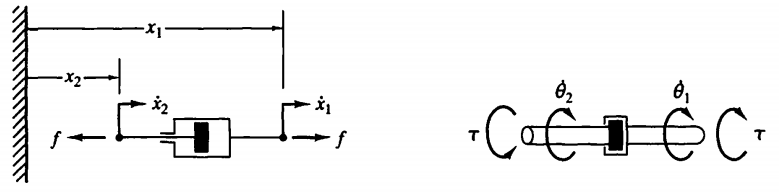
\includegraphics[width=\linewidth]{Damper.png}
  \caption{Translational and Torisional Dampers}
  \label{fig:boat1}
\end{figure}

$$F \propto (\dot{x_2} - \dot{x_1})$$
$$F \propto (\dot{\theta_2} - \dot{\theta_1})$$

The viscous friction coefficient is found emperically as follows: 
$$b = F/ (\dot{x_2} - \dot{x_1})$$
$$b = F/ (\dot{\theta_2} - \dot{\theta_1})$$
$$F = b(\dot{x_2} - \dot{x_1})$$
$$F = b(\dot{\theta_2} - \dot{\theta_1})$$

\subparagraph{Inertial Elements}~ \\
The mass of a system is also critical to its behavior. The translational velocity of an object is constant unless acted on by an outside force. The translational acceleration of an body is dependent on the objects mass and the magnitude of the force acting on the body. In translational motion, every point on the body moves through space. \\

$$F = ma$$

Analyzing rotational motion is more difficult. The rotational behavior of an object is dependent on the mass of the object AND the object mass distribution relative to a coordinate axis. This 'mass distribution' can be expressed as a scalar known as the 'moment of inertia'. In rotational motion, every point on the body moves except the axis of rotation. If you want the formulas for moment of inertia (J), look them up in a book. \\

$$\Sigma \tau = J \alpha$$

\subparagraph{Forced Response VS Natural Reponse}~ \\
System behavior is dependent on the systems initial conditions and inputs from the environment. A forced response is caused by a 'forcing function', which is a function describing system inputs from the environment. A natural response is due to initial conditions in the system. \\
Natural Response Example: A car is going down the road at steady 60 mph. At $t=0$, the engine cuts out. The car coasts down the road until it comes to a stop. The response after $t=0$ would be the natural response. \\
Forced Response Example: A car is going down the road. At $t=0$, the engine sets to a constant energy input into the car. This is a forced response. There is a user input forcing the behavior of the system. \\

\begin{figure}
\begin{center}
  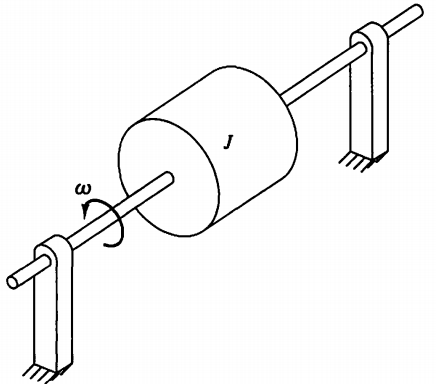
\includegraphics[width=20em]{Example_1}
  \caption{Translational and Torisional Dampers}
  \label{fig:boat1}
\end{center}
\end{figure}

\subparagraph{Example 1}~ \\

Lets consider a mass mounted to bearings as shown in the image. A person rotates the system until is reaches angular velocity $\omega(0)$ at $t=0$. At $t=0$, the person stops cranking the shaft of the system. Determine the behavior of the system. Note - This is an example of a natural response. 

\begin{align*}
\omega(0) &= \omega_0  &\text{Initial Conditions}\\
J\dot{\omega} &= -b\omega &\text{Equation of Motion}\\
J\dot{\omega} + b\omega &= 0 &\text{ } \\
\mathcal{L}(J\dot{\omega} + b\omega) &= \mathcal{L}(0)  &\text{Take the Laplace Transform}\\
J(s\mathcal{L}(\omega) - \omega(0)) + b \mathcal{L}(\omega)) &= 0 &\text{Use Laplace Substitution}\\
\mathcal{L}(\omega) &= \omega(0)\frac{1}{(s + \frac{b}{J})}  &\text{Solve Laplace Transform}\\
\mathcal{L}^{-1}(\mathcal{L}(\omega)) &= \mathcal{L}^{-1}\left(\omega(0)\frac{1}{(s + \frac{b}{J})}\right) &\text{Take the Inverse Laplce}\\
\omega(t) &= \omega(0)e^{-\left(\frac{b}{J}\right)t} &\text{Solution}\\
\end{align*}



%------------------------------------------------

\subsection{Heading on level 2 (subsection)}


\begin{align}
A = 
\begin{bmatrix}
A_{11} & A_{21} \\
A_{21} & A_{22}
\end{bmatrix}
\end{align}


%------------------------------------------------

\subsubsection{Heading on level 3 (subsubsection)}



\paragraph{Heading on level 4 (paragraph)}



%----------------------------------------------------------------------------------------
%	PROBLEM 2
%----------------------------------------------------------------------------------------

\section{Modeling Systems with Transfer-Functions}

%------------------------------------------------

\subsection{Example of list (3*itemize)}
\begin{itemize}
	\item First item in a list 
		\begin{itemize}
		\item First item in a list 
			\begin{itemize}
			\item First item in a list 
			\item Second item in a list 
			\end{itemize}
		\item Second item in a list 
		\end{itemize}
	\item Second item in a list 
\end{itemize}

%------------------------------------------------

\subsection{Example of list (enumerate)}

%----------------------------------------------------------------------------------------


\begin{figure}
  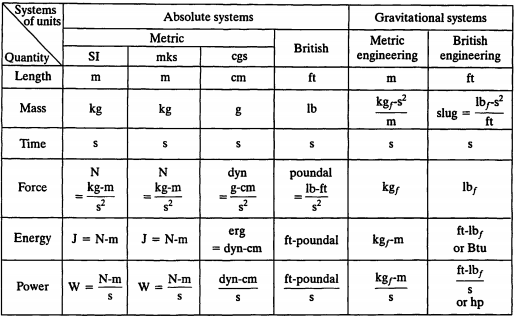
\includegraphics[width=40em]{System_of_Units.png}
  \caption{Systems of Units}
  \label{fig:boat1}
\end{figure}


\end{document}